\documentclass{article}

\usepackage[pdftex]{graphicx}
\usepackage[czech]{babel}
\usepackage[utf8]{inputenc}
\usepackage{enumitem}
\usepackage{amsmath}
\usepackage{url}
\usepackage{listings}
\usepackage{caption}
\usepackage[usenames,dvipsnames,svgnames,table]{xcolor}

\usepackage[pdftex]{hyperref}
\hypersetup{colorlinks=true,
  unicode=true,
  linkcolor=black,
  citecolor=black,
  urlcolor=black,
  bookmarksopen=true}

\usepackage[numbers,sort&compress]{natbib}

\newcommand*\justify{
  \fontdimen2\font=0.4em
  \fontdimen3\font=0.2em
  \fontdimen4\font=0.1em
  \fontdimen7\font=0.1em
  \hyphenchar\font=`\-
}

\author{Martin Úbl}

\title{KIV/OS - cvičení č. 4}

\begin{document}

\maketitle



\section{Obsah cvičení}

\begin{itemize}
	\item operační módy procesoru ARM1176
	\item tabulka vektorů přerušení
	\item IRQ
	\item driver pro ARM timer
\end{itemize}

\section{Operační módy procesoru ARM1176}

Procesor ARM1176 obsažený v mikrokontroléru BCM2835 je schopen operovat v několika módech, které se liší stupněm ochrany, sadou (uschovaných) registrů a určitými příznaky ve stavových registrech. Mód procesoru je určen spodními pěti bity v registru \texttt{CPSR}. Dodatečně ARM rozeznává implicitně ke každému režimu i úroveň ochrany (privilege level, \texttt{PL}), který definuje, k jakým zdrojům má program v čase vykonání jeho instrukcí přístup. Tento procesor má pouze 2 úrovně ochrany (neprivilegovaný \texttt{PL0} a privilegovaný \texttt{PL1}), ale ARM obecně může podporovat ještě jednu další pro virtualizaci (hypervizor, \texttt{PL2}).

\begin{itemize}
	\item \emph{user} -- uživatelský režim, ekvivalentní k uživatelskému režimu x86 (s CPL = 3), nesmí zasahovat do chráněných registrů, ani měnit úroveň ochrany procesoru
	\item \emph{FIQ} -- režim pro zpracování \emph{fast IRQ}, tedy hardwarových přerušení v \uv{rychlém} režimu (viz jiná cvičení nebo manuál)
	\item \emph{IRQ} -- režim pro zpracování hardwarových přerušení v běžném režimu
	\item \emph{supervisor} -- režim pro zpracování privilegovaných požadavků z uživatelského režimu, který je vyvolán buď při spuštění a resetu, nebo při zpracování instrukce \texttt{svc}
	\item \emph{abort} -- režim pro zpracování výjimek \emph{prefetch abort} a \emph{data abort}
	\item \emph{undefined} -- režim pro zpracování výjimek typu \emph{undefined instruction} (když je proveden pokus o dekódování neexistující instrukce)
	\item \emph{system} -- systémový režim, v podstatě podmnožina supervisor režimu, která ale používá stejnou sadu registrů jako \emph{user} režim -- hodí se tedy ke zpracování systémových tasků (bottom half přerušení, apod.), kdy je vyžadován přístup k privilegovaným prostředkům
	\item \emph{secure monitor} -- prostředek TrustZone modelu, ten ve cvičení probírat nebudeme
\end{itemize}

My budeme používat všechny režimy kromě \emph{FIQ} a \emph{secure monitor} režimu. V tomto cvičení se blíže podíváme na přerušení, a tedy režim \emph{IRQ}. V dalších cvičeních nás pak čeká přepnutí do \emph{user} módu (později i \emph{system} módu) pro vykonávání tasků, občasné přepnutí pro zpracování výjimek v \emph{abort} a \emph{undefined} módu a řízené přepínání do \emph{supervisor} módu kvůli zpracování systémových volání (\emph{supervisor call}, instrukce \texttt{svc}).

\section{Tabulka vektorů přerušení}

Stejně jako jiné architektury, tak i ARM podporuje mechanismus přerušení. Tabulka vektorů přerušení je pro běžný režim procesoru ARM1176 vždy situována na začátku adresovatelné paměti (s počátkem v 0x00000000). Každá položka tabulky má 4 bajty. Záznamem v tabulce je vždy spustitelný kód - programový čítač (\texttt{PC}) je vždy nastaven na příslušný offset v této tabulce, narozdíl od x86, kde je do \texttt{PC} nastavena až hodnota z této tabulky (tedy se provádí implicitně o krok navíc).

Z toho vyplývá, že do tabulky vektorů přerušení budeme chtít umístit nějakou instrukci skoku. Konkrétně budeme vkládat instrukci skoku na místo, kde se nachází skutečná obsluha daného typu přerušení. ARM rozeznává následující přerušení a očekává tyto offsety v tabulce:

\begin{description}
	\item[0x00] - reset -- vektor po resetu zařízení
	\item[0x04] - undefined instruction -- vektor při dekódování neznámé instrukce
	\item[0x08] - supervisor call -- vektor při volání supervisora
	\item[0x0C] - prefetch abort -- vektor při špatnému zásahu do paměti při pokusu o dekódování instrukce (do určité míry se překrývá s pojmem \uv{page fault})
	\item[0x10] - data abort -- vektor při špatném zásahu do paměti při pokusu o čtení dat
	\item[0x14] - nevyužito (v jiných procesorech jde o hypervisor call)
	\item[0x18] - IRQ -- hardwarové přerušení v \uv{běžném} režimu
	\item[0x1C] - FIQ -- hardwarové přerušení v \uv{rychlém} režimu
\end{description}

Mnemonický přepis tabulky by tedy mohl vypadat cca takto (ovšem zatím s velkým háčkem, viz níže):

\begin{lstlisting}
ldr pc, handle_reset
ldr pc, handle_undefined_instruction
ldr pc, handle_supervisor_call
...
ldr pc, handle_fiq
\end{lstlisting}

Tuto tabulku pak stačí při spuštění systému nakopírovat na začátek fyzické paměti, povolit přerušení a mělo by vše fungovat.

Problém ale nastává v momentě, kdy si uvědomíme, jak fungují takové skoky. Skoky při zpracování výjimek musí být absolutní a adresa v instrukci prozměnu relativní. Instrukce \texttt{ldr} totiž v případě modifikace programového čítače přejímá druhý operand jako adresu relativní právě k programovému čítači. Fakticky tedy na začátek paměti musíme nakopírovat jak tyto skokové instrukce, tak absolutní adresy obslužných procedur.

V instrukcích pak nebudou přímo návěští procedur, ale návěští, kde nalezneme skutečné absolutní adresy těchto procedur. Hlavní tabulku pak bude následovat právě tabulka absolutních adres.

Mnemonický přepis se pak změní na:

\begin{lstlisting}
ldr pc, handle_reset_ptr
ldr pc, handle_undefined_instruction_ptr
ldr pc, handle_supervisor_call_ptr
...
ldr pc, handle_fiq_ptr

handle_reset_ptr:
	.word handle_reset
handle_undefined_instruction_ptr:
	.word handle_undefined_instruction
handle_supervisor_call_ptr:
	.word handle_supervisor_call
...
handle_fiq_ptr:
	.word handle_fiq
\end{lstlisting}

Všechny položky tabulky vektorů přerušení se pak při překladu přeloží jako
\begin{lstlisting}
ldr	pc, [pc, #24]
\end{lstlisting}
jelikož offset od každé položky je konstantní.

Nyní by již skutečně vše mělo být připraveno. Tabulku hlavní i tabulku adres pak můžeme překopírovat například následovně:

\begin{lstlisting}
mov r0, #0x8000
mov r1, #0x0000

ldmia r0!,{r2, r3, r4, r5, r6, r7, r8, r9}
stmia r1!,{r2, r3, r4, r5, r6, r7, r8, r9}
ldmia r0!,{r2, r3, r4, r5, r6, r7, r8, r9}
stmia r1!,{r2, r3, r4, r5, r6, r7, r8, r9}
\end{lstlisting}

Instrukce \texttt{ldmia} a \texttt{stmia} slouží k hromadnému přesunu z adresy do registru a naopak. Vykřičník u bázového registru (\texttt{r0} a \texttt{r1}) znamená, že se má hodnota v registru posunout o finální hodnotu offsetu. Tato dvojice volání tedy, byť na první pohled vypadá stejně, ve výsledku operuje nad dvou po sobě jdoucích osmicích slov.

\section{IRQ}

IRQ (interrupt request) je externí hardwarové přerušení, které vyvolala nějaká periferie. V rámci BCM2835 to může být například časovač, GPIO řadič (resp. nějaký z pinů), Aux subsystém (UART, SPI) a jiné. Tato přerušení se musí vždy nejprve povolit na systémové úrovni a v příslušném subsystému povolit vyvolávání specifických přerušení.

Na systémové úrovni jde o bit 7 v řídicím registru \texttt{CPSR}. Ten je ve výchozím stavu zapnutý -- maskuje přerušení. To lze udělat ručně vyzvednutím registru \texttt{CPSR}, modifikací příslušného bitu a opětovným zapsáním:
\begin{lstlisting}
mrs r0, cpsr
bic r0, r0, #0x80
msr cpsr_c, r0
\end{lstlisting}
To je relativně zdlouhavé, mimo jiné i kvůli nemožnosti modifikovat řídicí registr přímo. Celý proces lze zjednodušit na jednu souhrnnou instrukci
\begin{lstlisting}
cpsie i
\end{lstlisting}
Instrukce typu \texttt{CPS} mění stav procesoru, zde konkrétně dochází k povolení přerušení (suffix \texttt{IE}), a to pouze běžných (jediný operand \texttt{i}). Z toho lze odvodit, jak bude vypadat mnemonický přepis instrukce pro maskování všech přerušení (\texttt{CPSID i}), nebo povolení FIQ (\texttt{CPSIE f}).

Pro ošetření IRQ pak můžeme definovat buď vstupní bod přímo v assembly a dodržet formát uvedený dříve, nebo můžeme funkci \texttt{irq\_handler} dekorovat atributem, který dá překladači hint o tom, že uvedená funkce je vstupním bodem ošetření výjimky:
\begin{lstlisting}
extern "C" void __attribute__((interrupt("IRQ"))) irq_handler()
{
  //
}
\end{lstlisting}
Tato funkce zůstane pro teď prázdná -- atribut kompilátoru řekne, že má společné chování pro handlery vložit automaticky. Pro teď nám to bude stačit, ale do dalších cvičení si tuto funkci tak jako tak přepíšeme do assembly, abychom měli úplnou kontrolu nad tím, co se kde děje.

V podstatě si je třeba uvědomit to, že při ošetřování výjimky typu IRQ se neuschovají některé z registrů. Jejich přepsáním by došlo ke změně stavu provádění kódu, který byl prováděn před vyvoláním výjimky, a tak je potřeba tyto registry uschovat. To je typicky provedeno na zásobník, který je pro IRQ režim vyhrazený vlastní.

My ho ale ještě nikde nevyhradili -- mělo bychom tedy jeden zásobník pro všechno a to není zrovna nejšťastnější řešení, a to jak z kapacitních důvodů, tak z bezpečnostních.

Do startovací rutiny proto doplňme vyhrazení zásobníků pro teď na pevně dané adresy v paměti. Budeme určitě potřebovat jeden zásobník pro IRQ, druhý pro FIQ a pak jeden pro supervisor mód. Využijeme toho, že můžeme volně mezi režimy přecházet změnou stavových bitů a nastavíme každý ze stack pointerů na námi zvolenou hodnotu. Pro přehlednost si definujme makra:
\begin{lstlisting}
.equ CPSR_MODE_FIQ, 0x11
.equ CPSR_MODE_IRQ, 0x12
.equ CPSR_MODE_SVR, 0x13
.equ CPSR_IRQ_INHIBIT, 0x80
.equ CPSR_FIQ_INHIBIT, 0x40
\end{lstlisting}
Zde máme pro módy IRQ, FIQ a SVR (supervisor) uložené hodnoty, které se lze dočíst v manuálu procesoru ARM. Dále definujeme hodnoty \texttt{CPSR} registru pro maskované IRQ a FIQ, jelikož máme v úmyslu přímo modifikovat obsah registru \texttt{CPSR} bez předchozího čtení.

Zásobníky pro IRQ a FIQ režimy jsou potřeba pouze velmi malé. Dejme tomu, že vyhradíme zásobníky s vrcholy \texttt{0x6000}, \texttt{0x7000} a \texttt{0x8000} pro IRQ, FIQ a supervisor režim. Toho docílíme velmi snadno:
\begin{lstlisting}
mov r0, #(CPSR_MODE_IRQ | CPSR_IRQ_INHIBIT | CPSR_FIQ_INHIBIT)
msr cpsr_c, r0
mov sp, #0x7000

mov r0, #(CPSR_MODE_FIQ | CPSR_IRQ_INHIBIT | CPSR_FIQ_INHIBIT)
msr cpsr_c, r0
mov sp, #0x6000

mov r0, #(CPSR_MODE_SVR | CPSR_IRQ_INHIBIT | CPSR_FIQ_INHIBIT)
msr cpsr_c, r0
mov sp, #0x8000
\end{lstlisting}

Všimněte si mimo jiné vkládání obsahu registru \texttt{R0} do \texttt{CPSR\_C} -- suffix \texttt{\_C} označuje dolních 8 bitů tohoto registru, a tedy zamezuje nechtěné modifikaci vyšších, stavových a indikačních bitů.

V tento moment tato implementace nepodporuje vnořená přerušení, ani se s nimi nijak nevypořádáváme v kódu. Nejjednodušším řešením je přerušení po čas vykonávání obsluhy zakázat a na jeho konci opět povolit (např. implicitně při vracení hodnoty \texttt{SPSR} do \texttt{CPSR}). S tím se ale vypořádáme jindy.

Teď přichází na řadu psaní ovladače pro řadič přerušení. Předtím prostudujme dokumentaci mikrokontroléru BCM2835. Tam se dozvíme, že IRQ jsou rozdělena na tzv. \emph{basic IRQ} a \uv{normální} IRQ. Ve skutečnosti jde o dva druhy IRQ dle zdroje. To, co je označeno jako basic IRQ jsou přerušení z periferií přímo obsažených ve specifikaci ARM procesoru. Zbylé přerušení jsou pro procesor externí a zahrnují například již zmíněný UART, SPI, I2C a další -- tedy takové periferie, které ARM nezná, ale jsou specifické pro mikrokontrolér BCM2835.

Nyní bychom měli definovat bázové adresy pro řadič přerušení, a nějaké výčtové typy identifikující zdroj přerušení -- to se dočteme v manuálu. Rozšiřme proto \texttt{peripherals.h} o další kód:

\begin{lstlisting}
constexpr unsigned long Interrupt_Controller_Base =
                         Peripheral_Base + 0x0000B200UL;

enum class Interrupt_Controller_Reg
{
  IRQ_Basic_Pending  = 0,
  IRQ_Pending_1      = 1,
  IRQ_Pending_2      = 2,
  FIQ_Control        = 3,
  IRQ_Enable_1       = 4,
  IRQ_Enable_2       = 5,
  IRQ_Basic_Enable   = 6,
  IRQ_Disable_1      = 7,
  IRQ_Disable_2      = 8,
  IRQ_Basic_Disable  = 9,
};

enum class IRQ_Basic_Source
{
  Timer              = 0,
  Mailbox            = 1,
  Doorbell_0         = 2,
  Doorbell_1         = 3,
  GPU0_Halt          = 4,
  GPU1_Halt          = 5,
  Illegal_Access_1   = 6,
  Illegal_Access_2   = 7,
};

enum class IRQ_Source
{
  AUX                = 29,
  I2C_SPI_SLAVE_INIT = 43,
  PWA_0              = 45,
  PWA_1              = 46,
  SMI                = 48,
  GPIO_0             = 49,
  GPIO_1             = 50,
  GPIO_2             = 51,
  GPIO_3             = 52,
  I2C                = 53,
  SPI                = 54,
  PCM                = 55,
  UART               = 57,
};
\end{lstlisting}

Z výše uvedeného a z manuálu se lze dočíst, že přerušení musíme nejprve povolit v příslušném registru nastavením bitu dané pefiferie na 1. Jelikož ARM nijak nesignalizuje při vyvolání externího přerušení co vlastně přerušení vyvolalo, je třeba projít všechny příznakové registry.

Pro povolení \uv{basic} přerušení nastavme příslušný bit v registru \texttt{IRQ\_Basic\_Enable}:

\begin{lstlisting}
void Enable_Basic_IRQ(IRQ_Basic_Source src)
{
  volatile unsigned long* regs =
     reinterpret_cast<unsigned long*>(Interrupt_Controller_Base);
     
  const int idx =
     static_cast<int>(Interrupt_Controller_Reg::IRQ_Basic_Enable);
     
  regs[idx] = 1 << static_cast<int>(src);
}
\end{lstlisting}

Analogicky lze odvodit kód pro zakázání přerušení z daného zdroje (výměnou registru za \texttt{IRQ\_Basic\_Disable}) a povolení a zakázání \uv{běžných} IRQ (výměnou registru za \texttt{IRQ\_Enable\_1} a \texttt{\_2}, resp. \texttt{IRQ\_Disable\_1} a \texttt{\_2}). Volba mezi registry 1 a 2 je opět po sadě 32 kanálů.

Nyní máme vše, co potřebujeme ke generickému zpracování přerušení (a IRQ) a můžeme se vrhnout na první periferii, od které budeme IRQ vyžadovat.

\section{ARM timer}

Timer je periferie, která se dá použít k časování. Klíčové je zde uvození slovy \uv{dá se použít}, jelikož to není explicitně jediný účel -- na mnoha embedded systémech se používá ke generování PWM signálu (Pulse Width Modulation; o té zase někdy jindy), nebo inverzně k čítání pulzů na nějakém vstupu. V podobě, ve které ho použijeme my, nám bude ale sloužit k časování.

Mikrokontrolér BCM2835 obsahuje dva druhy čítačů. Klasický (systémový) timer a pak ARM timer. My se teď budeme zabývat tím druhým -- jde o specifický druh časovače. ARM timer je ve své podstatě pouze čítač, který je na začátku inicializován hodnotou z \texttt{Load} registru a s nastavenou periodou je toto číslo dekrementováno až na nulu. Pokud je nastaveno opakované čítání, je znovu načtena hodnota registru \texttt{Load} a proces se opakuje. Časovač může při každém dosažení nuly vygenerovat přerušení. Časovač je řízen příznaky \texttt{Control} registru.

Frekvence čítání obecně je odvozena různými způsoby dle architektury -- někdy mají periferie vlastní časovací signál (a oscilátor), někdy je periferní časovací signál odvozen od taktovacího signálu procesoru, a tak podobně. V našem případě a případě ARM timeru je frekvence odvozena přímo od taktovací frekvence procesoru, a to pomocí softwarově nastavitelné předděličky. Ta dělí časovací signál buď číslem 1 (tedy nedělí), 16 nebo 256.

Rozhraní pro ARM timer se snaží dodržet rozhraní standardního čítače SP804. Proto je v dokumentaci BCM2835 něco trochu navíc a následně je připojena poznámka, že nastavení tohoto registru (bitu, hodnoty) nic nedělá. Základ ale skutečně z SP804 vychází a pro naše potřeby bude podporovaná podmnožina stačit.

Pro úspěšné rozběhání časovače a generování přerušení tedy musíme:
\begin{enumerate}
	\item nastavit \texttt{Load} registr na žádanou hodnotu
	\item nastavit \texttt{Control} registr příznaky, které od čítače chceme
	\item implementovat obsluhu přerušení časovače
		\begin{itemize}
			\item tady nesmíme zapomenout vymazat příznak čekajícího přerušení
		\end{itemize}
	\item nasměrovat generickou obsluhu přerušení do obsluhy přerušení časovače
\end{enumerate}

\subsection{Inicializace}

Pro lepší názornost ovládání \texttt{Control} registru si definujme jeho layout jako strukturu definovanou dle manuálu:
\begin{lstlisting}
struct TTimer_Ctl_Flags
{
  uint8_t unused_0 : 1;
  uint8_t counter_32b : 1;
  uint8_t prescaler : 2;
  uint8_t unused_1 : 1;
  uint8_t interrupt_enabled : 1;
  uint8_t unused_2 : 1;
  uint8_t timer_enabled : 1;
  uint8_t halt_in_debug_break : 1;
  uint8_t free_running_enable : 1;
  uint16_t unused_3 : 10;
  uint16_t free_running_prescaler : 16;
  uint16_t unused_4 : 10;
};
\end{lstlisting}
\emph{Pozn. 1: v manuálu BCM2835 je překlep -- ve skutečnosti je čítač v 16 nebo 32-bitovém módu, nikoliv 23-bitovém, jak uvádí příslušná sekce v manuálu.}\\
\emph{Pozn. 2: pozor na padding -- v případě nutnosti obalme strukturu příslušnou packing direktivou.}
\\

Nyní opět rozšiřme \texttt{peripherals.h} soubor o nové adresy a registry:
\begin{lstlisting}
constexpr unsigned long Timer_Base =
              Peripheral_Base + 0x0000B400UL;

enum class Timer_Reg
{
  Load          = 0,
  Value         = 1,
  Control       = 2,
  IRQ_Clear     = 3,
  IRQ_Raw       = 4,
  IRQ_Masked    = 5,
  Reload        = 6,
  Pre_Divider   = 7,
  Free_Running  = 8,
};
\end{lstlisting}

Pro potřeby manipulace s časovačem vytvořme pomocnou funkci pro přístup k registrům (jen předá adresu registru tak, abychom kód nezaplevelili zbytečnými type-casty):
\begin{lstlisting}
volatile uint32_t& Timer_Register(Timer_Reg reg)
{
  volatile unsigned long* regs =
      reinterpret_cast<unsigned long*>();

  return regs[static_cast<int>(reg)];
}
\end{lstlisting}
Kód pro samotnou inicializaci pak může vypadat třeba takto:
\begin{lstlisting}
void Enable_Timer(uint32_t load, uint32_t prescaler)
{
  Timer_Register(Timer_Reg::Load) = load;
  
  TTimer_Ctl_Flags reg;
  reg.counter_32b = 1;
  reg.interrupt_enabled = 1;
  reg.timer_enabled = 1;
  if (prescaler == 16)
    reg.prescaler = 0b01;
  else if (prescaler == 256)
    reg.prescaler = 0b10;
  else
    reg.prescaler = 0b00;
    
  Timer_Register(Timer_Reg::Control) =
      *reinterpret_cast<unsigned int*>(&reg);
      
  Timer_Register(Timer_Reg::IRQ_Clear) = 1;
}
\end{lstlisting}
Výše uvedený kód je pochopitelně uveden jako příklad, kde není odchyceno spousty jiných, potenciálně chtěných variant. Další rozšíření ovladače pro časovač je ponecháno čtenáři jako cvičení -- můžete například definovat výčet pro hodnotu předděličky, celý ovladač zavřít do třídy (jako GPIO ovladač) a inicializovat konstruktorem bázovou adresu pro registry, lze pak dodělat flexibilnější nastavování registrů, přidat výpočet intervalů (aby nemusel uživatel zadávat hodnotu registru a děličku) a tak dále. Pro teď ale tyto speciality vynechme a věnujme se obecným principům.

\subsection{Obsluha přerušení}

V první řadě definujme samotnou obsluhu -- ta bude velice jednoduchá. Půjde jen o funkci, kde vynulujeme bit reprezentující čekající přerušení, a pak dáme prostor pro specifické funkce, které chceme při přerušení časovače vykonávat:

\begin{lstlisting}
void Handle_Timer_IRQ()
{
  Timer_Register(Timer_Reg::IRQ_Clear) = 1;
  
  // tady muzeme delat neco konkretniho
  // ... zatim ale nemame co
}
\end{lstlisting}

Poté by bylo dobré mít možnost, jak se zeptat ovladače pro časovač, zda se má obsluha vůbec volat z generické obsluhy:

\begin{lstlisting}
bool Is_Timer_IRQ_Pending()
{
  return Timer_Regs(Timer_Reg::IRQ_Masked);
}
\end{lstlisting}
\emph{Pozn.: pro zjištění by šel použít i registr \texttt{IRQ\_Raw} -- ten ale nezohledňuje to, zda jsou přerušení časovače vůbec povolená.}

Nyní můžeme obohatit generickou obsluhu přerušení o podmíněné volání obsluhy IRQ časovače:
\begin{lstlisting}
extern "C" void __attribute__((interrupt("IRQ"))) irq_handler()
{
  if (Is_Timer_IRQ_Pending())
    Handle_Timer_IRQ();
}
\end{lstlisting}

Nyní by mělo vše fungovat jak má -- máme funkční časovač, kterým můžeme načasovat nějakou událost. Toho využijeme hned v příštím cvičení, ve kterém implementujeme preemtivní round-robin plánovač.

\section{Úkol za body}

Ještě než budeme implementovat plánovač bychom si měli osvojit funkci časovače a získat představu o tom, jakého rozlišení lze dosahnout.

Obsahem úkolu za body bude blikání indikační LED (ACT LED nebo ta na rozšiřující desce). Využijte jednak driver pro GPIO a jednak driver pro časovač. Vámi vybranou LED blikejte tak, že bude 1 vteřinu rozsvícena na plný svit, 1 vteřinu zhasnuta, a pak bude 2 vteřiny rozsvícena na polovinu svitu a zase 1 vteřinu zhasnuta. Celý cyklus se bude opakovat.

Jak docílit polovičního svitu? Buď to vyžaduje alespoň povrchní znalosti elektrotechniky, nebo stačí prostě přijmout jednoduchý fakt -- když budeme LED rychle rozsvěcet a zhasínat s určitou relativně vysokou frekvencí, a když pro stav \uv{zhasnuto} (resp. \uv{rozsvíceno}, dle druhu LED) vyhradíme trochu delší čas, tak se LED nerozsvítí naplno.

\begin{figure}[ht!]
	\centering
	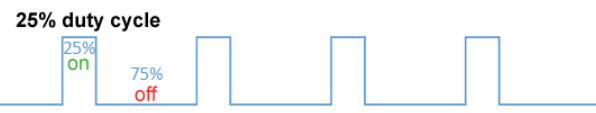
\includegraphics[width=\linewidth]{pwm.png}
	\caption{Konkrétní případ pulzně-šířkové modulace, zde jako příklad, jak docílit menšího svitu LED; výřez převzat z \url{https://en.wikipedia.org/wiki/Pulse-width_modulation}}
\end{figure}

Pokuste se minimalizovat zbytečné probouzení -- periodu časovače (\texttt{Load} a předděličku) nastavte tak, aby odpovídala potřebnému času, pokud to je možné (v případě vteřinového plného výkonu nebo zhasnuté LED; v případě polovičního svitu to dále minimalizovat pouze za použití software nejde).

\emph{Pozn. 1: minimalizace zbytečného probouzení je pak klíčovou věcí při minimalizaci spotřeby elektrické energie (maximalizace výdrže na bateriovém napájení). To je něco, co od zařízení jako je RPi Zero (a jeho software) jednoznačně vyžadujeme.}\\
\emph{Pozn. 2: polovičního svitu LED lze dosahnout i použitím mechanismu PWM, který RPi Zero taktéž obsahuje. O tom ale jindy.}

\end{document}























